\chapter{Vektoren}

\section{Einführung}
Den Begriff des \textit{Vektors} kennen Sie bereits aus dem Physikunterricht. Wir wiederholen das Wichtigste. Zunächst betrachten wir die mathematische Definition eines Vektors:

\begin{definition}\index{Vektor}
Ein Vektor entspricht der Menge aller Pfeile mit gleicher
Richtung und gleicher Länge.
Ein einzelner Pfeil ist ein sogenannter Repräsentant des
entsprechenden Vektors.

\end{definition}
Wir schreiben Vektoren üblicherweise so:
\[ \vv{r} = \vv{AB} \]
also mit Anfangs- und Endpunkt oder mit Kleinbuchstaben.

\begin{definition}\index{Gegenvektor}
Der Gegenvektor $-\vv{r}$ zu einem Vektor $\vv{r}$ ist der Vektor mit gleicher Länge aber entgegengesetzter Richtung. Es gilt:
\[ \vv{AB} = \vv{r} \]
\[ \vv{BA} = -\vv{r} \]
\[ \vv{BA} = -\vv{AB} \]
\end{definition}

\begin{definition}\index{Skalar}
Ein Skalar ist eine mathematische Grösse, die allein durch die Angabe eines Zahlenwertes charakterisiert ist, also im Allgemeinen eine reelle Zahl.
\end{definition}

Wir betrachten als nächstes die Grundoperationen zum rechnen mit Vektoren:
\begin{theorem}[Vektorsumme]
Für die Vektorsumme $\vv{a} + \vv{b} = \vv{AB} + \vv{CD}$ gilt:
\[ \vv{a} + \vv{b} = \vv{AD} \]
\end{theorem}
Der Anfangspunkt des 2. Vektors wird an den Endpunkt des
1. Vektors angefügt. Es gilt das Kommutativgesetz nach dem Vektorparallelogramm. 

\begin{theorem}[Vektordifferenz]
Für die Vektordifferenz $\vv{a} - \vv{b} = \vv{AB} - \vv{CD}$ gilt:
\[ \vv{a} - \vv{b} = \vv{a} + (-\vv{b}) = \vv{AC} \]
\end{theorem}
Dies kann also als Addition des Gegenvektors von $\vv{b}$ aufgefasst werden.

\begin{theorem}[Skalare Multiplikation]
\[ \lambda \cdot \vv{a} = \vv{\lambda a} \]
Ist $s>0$, so haben $\vv{a}$ und $\vv{\lambda a}$ die gleiche Richtung,
ist $s<0$, so haben sie die entgegengesetzte Richtung.
\end{theorem}
Mit Vektoren darf man rechnen wie mit algebraischen Termen (Zahlen und Variablen) ausser bei der
Division darf im Divisor kein Vektor sein.

\begin{exercises}



%\begin{multicols}{2}
\begin{exercise}
Die Vektoren $\vv{a}$, $\vv{b}$ und $\vv{c}$ sind gegeben, wobei gilt: $a=2cm$, $b=2.5cm$, $c=3cm$ und $\vv{a}$ ist rechtwinklig zu $\vv{b}$. $\vv{b}$ und $\vv{c}$ stehen in einem Winkel von \SI{30}{degree} zu einander.
Konstruieren Sie den Vektor:
\begin{enumerate}
\item[(a)]  $\vv{u} = 2 \vv{a} + \vv{b} - 4 \vv{c}$
\item   $\vv{v}$ so, dass: $3 \vv{a} - 2 \vv{b} + 3 \vv{c} + \vv{v} = 0$
\item $\vv{w}$ so, dass: $ \vv{a} +3 \vv{b} -4 \vv{c} + 2 \vv{w} = 0$
\end{enumerate}
\begin{answer}

\end{answer}
\end{exercise}

\begin{exercise}
Ein Dreieck $ABC$ ist gegeben durch $\vv{AB}=\vv{c}$ und $\vv{BC}=\vv{a}$.
Der Punkt $D$ ist Mittelpunkt der Seite $AB$.
Drücken Sie die Vektoren $\vv{AC}$, $\vv{AD}$ und $\vv{CD}$ durch $\vv{a}$ und $\vv{c}$ aus.

\begin{answer}
$\vv{AC} = \vv{c} + \vv{a}$
$\vv{AD} = \frac{1}{2} \vv{c}$
$\vv{CD} = - \vv{a} - \frac{1}{2} \vv{c}$
\end{answer}
\end{exercise}

\begin{exercise}
Ein Parallelogramm $ABCD$ ist mit $\vv{AB}=\vv{a}$ und $\vv{BC}=\vv{b}$ gegeben.
Der Punkt $E$ ist Mittelpunkt von $\vv{AB}$;
$F$ liegt auf $BC$ so, dass $BF:FC=3:2$ gilt.
Drücken Sie die Vektoren $\vv{AE}$, $\vv{AC}$, $\vv{BD}$, $\vv{CD}$, $\vv{DE}$, $\vv{BF}$, $\vv{AF}$ und $\vv{EF}$ durch $\vv{a}$ und $\vv{b}$ aus.
\begin{answer}
$\vv{AE} = \frac{1}{2} \vv{a}$ 
$\vv{AC} = \vv{a} + \vv{b}$
$\vv{BD} = -\vv{a} + \vv{b}$  
$\vv{CD} = -\vv{a}$
 $\vv{DE}= -\vv{b} + \frac{1}{2} \vv{a}$
$\vv{BF} = \frac{3}{5} \vv{b}$
$\vv{AF} = \vv{a} +\frac{3}{5} \vv{b}$
$\vv{EF} = \frac{1}{2} \vv{a} +\frac{3}{5} \vv{b}$
\end{answer}
\end{exercise}

\begin{exercise}
Welche besondere Lage haben die folgenden Punkte?
\begin{enumerate}
\item[(a)] $A(x|0|0)$
\item $B(x|y|0)$
\item $C(x|0|z)$
\item $D(0|y|4)$
\item $E(3|y|z)$
\item $F(x|2|z)$
\item $G(x|1|1)$
\item $H(0|a|a)$
\end{enumerate}
\begin{answer}
$A$ liegt auf der $x$-Achse: 0 Abweichung in Richtung $y$ und $z$
$B$ liegt in der $xy$-Ebene: 0 Abweichung nach oben
$C$ liegt in der $xz$-Ebene: 0 Abweichung in Richtung $y$-Achse
$D$ liegt in der $yz$-Ebene: 0 Abweichung Richtung $x$-Achse
und zwar auf einer Parallelen zur $y$-Achse auf der Höhe 4
$E$ liegt in einer Parallelebene zur $yz$-Ebene 3 weiter vorne
$F$ liegt in einer Parallelebene zur $xz$-Ebene um 2 weiter rechts
$G$ liegt auf einer Parallelen zur $x$-Achse durch den Punkt $( 0 | 1 | 1 )$.
$H$ liegt auf der Winkelhalbierenden in der $yz$-Ebene durch $( 0 | 0 | 0 )$ und $( 0 | 3 | 3 )$
\end{answer}
\end{exercise}

%\end{multicols}
\end{exercises}

\section{Kollineare und komplanare Vektoren, Basis}
\begin{definition}\index{kollinear, komplanar}
Vektoren heissen \textit{kollinear}, bzw. \textit{komplanar}, wenn ihre Repräsentanten parallel zu \textit{einer} Geraden bzw. parallel zu \textit{einer} Ebene sind.
\end{definition}

Der Nullvektor $\vv{0}$ wird zu jedem anderen Vektor sowohl als kollinear wie auch als komplanar angesehen. Zwei Vektoren sind stets komplanar, jedoch sind sie im Allgemeinen nicht kollinear.

\begin{marginfigure}
    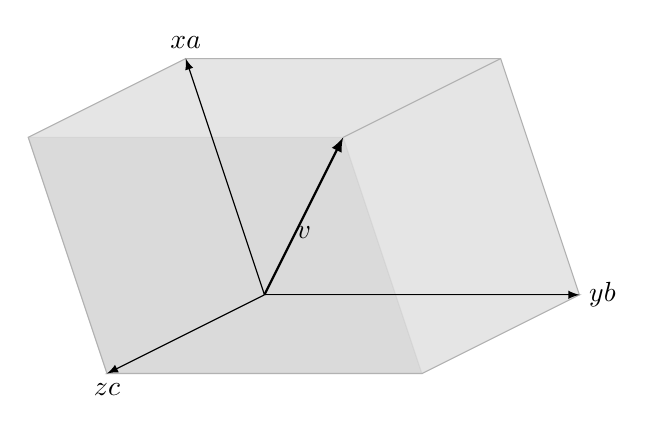
\begin{tikzpicture}
        \draw[gray!60, fill=gray!20] (0,0) -- (4,0) -- (3,3) -- (-1,3) --cycle;
        \draw[gray!60, fill=gray!20] (0,0) -- (4,0) -- (2,-1) -- (-2,-1) --cycle;
        \draw[gray!60, fill=gray!20] (0,0) -- (-1,3) -- (-3,2) -- (-2,-1) --cycle;
        \draw[gray!60, fill=gray!60, opacity=.2] (-3,2) -- (1,2) -- (2,-1) -- (-2,-1) --cycle;
        \draw[gray!60] (1,2) -- (3,3);
        \draw[-latex] (0,0) -- (4,0) node[right] {$y\vv{b}$};
        \draw[-latex] (0,0) -- (-1,3)  node[right, above] {$x\vv{a}$};
        \draw[-latex] (0,0) -- (-2,-1) node[below] {$z\vv{c}$};
        \draw[thick, -latex] (0,0) --node[below]{$\vv{v}$} (1,2);
        
    \end{tikzpicture}
\end{marginfigure}
Wir betrachten nun drei feste, nicht komplanare Vektoren $\vv{a}$, $\vv{b}$ und $\vv{c}$ sowie einen weiteren Vektor $\vv{v}$ der Form $\vv{v} = x \vv{a} + y \vv{b} + z \vv{c}$. Man sagt, $\vv{v}$ sein eine \textit{Linearkombination} von $\vv{a}$, $\vv{b}$ und $\vv{c}$. Diese Linearkombination kann man sich räumlich so vorstellen: Man denkt sich die drei Vektoren $\vv{a}$, $\vv{b}$ und $\vv{c}$ von einem gemeinsamen Ausgangspunkt $O$ aus repräsentiert. Jeweils zwei der repräsentierenden Pfeile legen dann eine Ebene fest (in der sie liegen). Werden diese Ebenen wier in der Skizze rechts je parallel durch die Pfeilspitzen der Repräsentanten von $x \vv{a}$, $y \vv{b}$ und $z \vv{c}$verschoben, so entsteht ein Spat (Pendant zum Parallelogramm im zweidimensionalen Fall). Der Körperdiagonalen-Pfeil mit Ausgangspunkt $O$ repräsentiert denn $\vv{v}$. Umgekehrt ist es nach Vorgabe der Vektoren $\vv{a}$, $\vv{b}$ und $\vv{c}$ mit dieser Spatkonstruktion jederzeit möglich, die Zahlenfaktoren $x$, $y$ und $z$ eindeutig aufzufinden.

\begin{mainTheorem}[Basissatz]\label{theorem:basis}
Für 4 Vektoren $\vv{a}$, $\vv{b}$, $\vv{c}$ und $\vv{v}$, bei denen die ersten 3 nicht komplanar sind, existiert stets eine Darstellung $\vv{v} = x \vv{a} + y \vv{b} + z \vv{c} $ mit eindeutigen Zahlen $x$, $y$ und $z$. Kurz: $\vv{v}$ lässt sich stets als Linearkombination von $\vv{a}$, $\vv{b}$ und $\vv{c}$ schreiben.
\end{mainTheorem}

\begin{definition}\index{Basis}
Die drei vorgegebenen, nicht komplanaren Vektoren $\vv{a}$, $\vv{b}$ und $\vv{c}$ werden als Basisvektoren oder kurz \textit{Basis} bezeichnet; sie legen drei Richtungen im dreidimensionalen Raum fest.
\end{definition}
Die Möglichkeit jeden beliebigen Vektor $\vv{v}$ in der Form $\vv{v} = x \vv{a} + y \vv{b} + z \vv{c} $, d.h. als Linearkombination der Basisvektoren darstellen zu können, ist von zentraler Bedeutung. Dadurch lässt sich nämlich jeder Vektor algebraisch beschreiben, und zwar durch die drei eindeutig festgelegten Zahlen $x$, $y$ und $z$, welche die ``Ausdehnungen'' des Vektors in Richtung der drei Basisvektoren angeben. Im Folgenden werden wir uns allerdings nicht auf eine beliebige Basis beziehen, sondern auf eine sehr spezielle, nämlich eine sogenannt orthonormierte. Bei dieser speziellen Wahl der basis werden gewisse algebraische Beschreibungen viel einfacher als bei einer beliebigen Basis. 

\section{Vektoren und Punkte im Koordinatensystem}

\begin{definition}\index{Koordinatensystem}
Ein \textit{orthogonales Rechtssystem}, kurz \textit{Koorinatensystem}, besteht aus einem festen Punkt $O$, dem Urpsrung, und drei nummerierten, nicht komplanaren Vektoren $\vv{e_{1}}$, $\vv{e_{2}}$ und $\vv{e_{3}}$, den \textit{Basisvektoren}, die folgende drei Bedingungen erfüllen:
\begin{itemize}
\item Ihre Repräsentanten mit Anfangspunkt $O$ stehen paarweise senkrecht aufeinander (``ortho'')
\item Ihre Beträge sind je 1, d.h. es sind sogenannte Einheitsvektoren (``normiert'')
\item Ihre Orientierung entspricht jener der drei gepsreizten Finger Daumen  ($\vv{e_{1}}$), Zeigefinger ($\vv{e_{2}}$) und Mittelfinger ($\vv{e_{3}}$) der rechten Hand. Man sagt: $\vv{e_{1}}$, $\vv{e_{2}}$ und $\vv{e_{3}}$ bilden in dieser Reihenfolge ein Rechtssystem.
\end{itemize}
\end{definition}

Allen nachfolgenden Betrachtungen liegt stets ein Koordinatensystem mit den obgenannten
Eigenschaften und Bezeichnungen zugrunde.
Aufgrund des Satzes \ref{theorem:basis} ist jeder Vektor eine Linearkombination der Basisvektoren: $\vv{v} = x \vv{e_{1}} + y \vv{e_{2}} + z \vv{e_{3}}$
\begin{definition}\index{Komponenten eines Vektors}
Die Koeffizienten $x$,$y$ und $z$ der Linearkombination $\vv{v} = \vv{e_{1}} + \vv{e_{2}} + \vv{e_{3}}$ heissen die \textit{Komponenten} von $\vv{v}$. Man schreibt abgekürzt $\vv{v} = \Vek{x}{y}{z}$ und spricht von der \textit{Komponentendarstellung} von $\vv{v}$.
\end{definition}
Für die Basisvektoren gilt speziell: $\vv{e_{1}} = \Vek{\qquad}{\qquad}{\qquad}$, $\vv{e_{2}} = \Vek{\qquad}{\qquad}{\qquad}$, $\vv{e_{3}} = \Vek{\qquad}{\qquad}{\qquad}$

\subsection{Rechnen mit Komponenten}

\begin{example}
Der Nullvektor:
\[ \vv{0} = \Vek{\qquad \qquad}{\qquad \qquad}{\qquad \qquad} \]
Beweis:
\[ \vv{0} = 0\vv{e_{1}} + 0\vv{e_{2}} + 0\vv{e_{3}} \]
\end{example}

\begin{example}
Der Gegenvektor:
\[ \vv{a} = \Vek{a_{1}}{a_{2}}{a_{3}} \qquad \Leftrightarrow \qquad -\vv{a} = \Vek{\qquad \qquad}{\qquad \qquad}{\qquad \qquad} \]
Beweis:
\[ \vv{a} = a_{1} \vv{e_{1}} + a_{2} \vv{e_{2}} + a_{3} \vv{e_{3}}  \qquad \Leftrightarrow \qquad -\vv{a} = -(a_{1} \vv{e_{1}} + a_{2} \vv{e_{2}} + a_{3} \vv{e_{3}}) \]
Durch Umformen: 
\[ -\vv{a} = (-a_{1}) \vv{e_{1}} + (-a_{2}) \vv{e_{2}} + (-a_{3}) \vv{e_{3}} = \Vek{\qquad \qquad}{\qquad \qquad}{\qquad \qquad} \]
\end{example}

\begin{example}
Der Betrag eines Vektors:
\[|\vv{a}| = \left\vert \Vek{a_{1}}{a_{2}}{a_{3}} \right\vert = \qquad \qquad \qquad \]
Beweis:
\[|\vv{a}| =\sqrt{(\sqrt{|a_{1}|^{2} + |a_{2}|^{2} })^{2}+ |a_{3}|^{2}} \]
\[ = \sqrt{|a_{1}|^{2} + |a_{2}|^{2}+ |a_{3}|^{2}} = \]
(zweimal Satz von Pythagoras)
\end{example}

\begin{example}
Addition und Subtraktion:
\[ \Vek{a_{1}}{a_{2}}{a_{3}} \pm \Vek{b_{1}}{b_{2}}{b_{3}} = \Vek{a_{1} \pm b_{1}}{a_{2} \pm b_{2}}{a_{3} \pm b_{3}} \]
Beweis:
\vspace{3cm}
\end{example}

\begin{example}
Multiplikation eines Vektors mit einer Zahl:
\[ x \Vek{a_{1}}{a_{2}}{a_{3}} = \Vek{x a_{1}}{x a_{2}}{x a_{3}} \]
Beweis:
\vspace{3cm}
\end{example}

\begin{exercisesKapitel}


\begin{exercise}
Vereinfachen Sie:
\[ \frac{1}{2} \vv{a} - ( \frac{2}{3} \vv{b} - \vv{c} - ( \frac{1}{3} \vv{b} - \vv{c}) + \frac{1}{2} \vv{a})+ \frac{1}{3} \vv{b} \]
\end{exercise}

\begin{exercise}
Lösen SIe nach $\vv{x}$ auf:
\[ \frac{1}{3} ( 2\vv{x}-\vv{b}+\vv{c})=2\vv{b}+\frac{1}{2}(\vv{x}+2\vv{b}-3\vv{c})\]
\end{exercise}

\begin{exercise}
Wählen Sie zwei nicht kollineare Vektoren $\vv{a}$ und $\vv{b}$ und illustrieren Sie mit einer Skizze das Distributivgesetz:
\[x (\vv{a} + \vv{b}) = x \vv{a} + x \vv{b} \]
\end{exercise}

\begin{exercise}
Gegeben ist ein Parallelogramm $ABCD$ mit Diagonalenschnittpunkt $M$. Stellen Sie folgende Vektoren als Linearkombination von $\vv{a} = \vv{AB}$ und $\vv{b} = \vv{AD}$ dar:
\begin{enumerate}
\item $\vv{AC}$
\item $\vv{DA}$
\item $\vv{BD}$
\item $\vv{¨BM}$
\item $\vv{MA}$
\end{enumerate}
\end{exercise}


\begin{exercise}
Beutreilen Sie, wahr (w) oder falsch (f)?
\begin{enumerate}
\item Zwei Vektoren sind stets kollinear
\item Zwei Vektoren sind stets komplanar
\item Kollineare Vektoren sind stets komplanar
\item Zwei Vektoren sind genau dann kollinear, wenn einer der beiden ein Vektorvielfaches des andern ist
\end{enumerate}
\end{exercise}

\begin{exercise}
Formulieren Sie folgende Implikation umgngssprachlich:
\[ \vv{a} = -\vv{b} \Rightarrow |\vv{a}| = |\vv{b}|\]
\end{exercise}

\begin{exercise}
Notieren Sie formal:
Wird ein Vektor mit dem Kehrwert seines Betrags multipliziert, so entsteht ein Vektor, dessen Betrag gleich 1 ist.
\end{exercise}

\end{exercisesKapitel}

\begin{marginfigure}[1cm]
    \tdplotsetmaincoords{60}{110}
    \begin{tikzpicture}[scale=1, tdplot_main_coords, vektor/.style={-stealth,very thick}]
        \draw[->,thick] (0,0,0) -- (4,0,0) node[anchor=west]{$x$};
	    \draw[->,thick] (0,0,0) -- (0,4,0) node[anchor=west]{$y$};
	    \draw[->,thick] (0,0,0) -- (0,0,4) node[anchor=west]{$z$};
	    \coordinate (O) at (0,0,0);
	    \tdplotsetcoord{P}{4}{55}{65}
	    \draw[vektor] (O) --node[above] {$\vv{OP}$} (P) node[above] {$P$};
	    \draw[dashed] (O) -- (Pxy);
	    \draw[dashed] (Pxy) -- (P);
    \end{tikzpicture}

\caption{Der Punkt $P$ und der dazugehörende Ortsvektor $\vv{OP}$.}

\end{marginfigure}

\section{Koordinatendarstellung von Punkten}
Bei der Definition des Koordinatensystems haben wir den Ursprung $O$ eingeführt. Für die Komponentendarstellung von Vektoren wäre dies aber nicht nötig, da Vektoren nicht ``ortsgebunden'' sind. Für die Koordinatendarstellung von Punkten ist jedoch der Ursprung $O$ unerlässlich.

Zwischen Vektoren und Punkten besteht eine umkehrbar eindeutige Zuordnung, die bei der nachfolgenden Definition der Koordinatendarstellung von Punkten benutzt wird. Ist ein Vektor durch den Pfeil repräsentiert, der vom Ursprung $O$ ausgeht ($O$ ist Anfangspunkt) und bezeichnet $P$ die Pfeilspitze ($P$ ist Endpunkt), so lässt sich diese Zuordnungwie folgt schreiben:
\[ \text{Vektor } \vv{OP} \leftrightarrow \text{Punkt } P \]
\begin{definition}\index{Koordinaten}
Die Komponenten $x$, $y$, $z$ von $\vv{OP}= \Vek{x}{y}{z}$ heissen die \textit{Koordinaten} von $P$.
\end{definition}
Man schreibt $P=(x/y/z)$ und spricht von der \textit{Koordinatendarstellung} von $P$. Der Vektor $\vv{OP}$ heisst \textit{Ortsvektor} des Punktes $P$

\begin{warning}
Trotz der engen Beziehung zwischen Punkten und ihren Ortsvektoren sollte man nie Punkte ``addieren'' oder ``subtrahieren''. Überdies ist der Unterschied in der Schreibweise zwischen geometrisch verschiedenen Objekten, Vektoren und Punkten, konsequent zu beachten (Koordinaten von Punkten schreiben wir nebeneinander, Komponenten von Vektoren übereinander).
\end{warning}



Nennen Sie die Koordinatendarstellungen der im nebenstehenden Koorinatensystem gezeichneten Punkten.

\begin{example}
Geben Sie den Verbindungsvektor $\vv{AB}$ der Punkte $A$ und $B$ an.
\[ A = (a_{1}/a_{2}/a_{3}) \]
\[ B = (b_{1}/b_{2}/b_{3}) \]
\end{example}
\begin{marginfigure}
    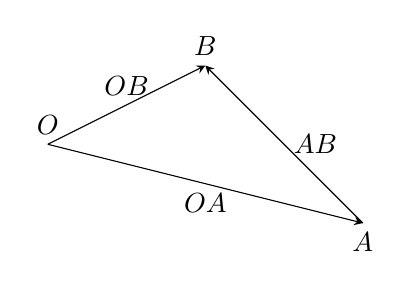
\begin{tikzpicture}
        \draw[-stealth] (0,0) node[above] {$O$} --node[above] {$\vv{OB}$} (2,1) node[above] {$B$};
        \draw[-stealth] (0,0) -- node[below] {$\vv{OA}$} (4,-1) node[below] {$A$};
        \draw[-stealth] (4,-1) -- node[right] {$\vv{AB}$ } (2,1);
        
    \end{tikzpicture}
\end{marginfigure}
\begin{solution}
Wegen $\vv{AB} = \vv{OB}-\vv{OA}$ gilt:
\[ \vv{AB} = \Vek{b_{1}-a_{1}}{b_{2}-a_{2}}{b_{3}-a_{3}} \]
\textit{Kurz: Koordinaten des Endpunktes minus entsprechende Koordinaten des Anfangspunktes!}
\end{solution}

\begin{example}
Geben Sie die Streckenlänge $\overline{AB}$ an.
\[ A = (a_{1}/a_{2}/a_{3}) \]
\[ B = (b_{1}/b_{2}/b_{3}) \]
\end{example}

\begin{solution}
Wegen $\overline{AB} = |\vv{AB}|$ gilt:
\[ \overline{AB} = \sqrt{(b_{1}-a_{1})^{2} + (b_{2}-a_{2})^{2} + (b_{3}-a_{3})^{2}} \]
\end{solution}

\begin{example}
Geben Sie die Streckenmitte $M$ von $AB$ an.
\[ A = (a_{1}/a_{2}/a_{3}) \]
\[ B = (b_{1}/b_{2}/b_{3}) \]
\end{example}

\begin{solution}
Wegen 
\[ \vv{OM} = \vv{OA} + \frac{1}{2} \vv{AB} = \Vek{a_{1}}{a_{2}}{a_{3}} + \frac{1}{2} \Vek{b_{1}-a_{1}}{b_{2}-a_{2}}{b_{3}-a_{3}} = \Vek{a_{1} + \frac{1}{2} (b_{1} - a_{1})}{a_{2} + \frac{1}{2} (b_{2} - a_{2})}{a_{3} + \frac{1}{2} (b_{3} - a_{3})} = \Vek{\frac{1}{2} (a_{1} + b_{1})}{\frac{1}{2} (a_{2} + b_{2})}{\frac{1}{2} (a_{3} + b_{3})}\] gilt: 
\[ M = \left( \frac{a_{1}+b_{1}}{2} / \frac{a_{2}+b_{2}}{2} / \frac{a_{3}+b_{3}}{2} \right) \]
Also das arithmetische Mittel der entsprechenden Koordinaten!
\end{solution}

%%%%%%%%%%%%%%%%%% Übungen %%%%%%%%%%%%%%%%%%%

\begin{exercisesKapitel} 
\setcounter{exercise}{7}
\begin{exercise}
$A=(1/-2/3)$, $B=(5/2/-5)$, $C=(9/6/-7)$ \newline
Bestimmen Sie die Seitenmittelpunkte und den Schwerpunkt des Dreiecks $ABC$. (Der Schwerpunkt des Dreiecks ist der Schnittpunkt der drei Seitenhalbierenden, er teilt die Seitenhalbierenden in Abschnitte mit dem Längenverhältnis 1:2).
\begin{answer}
Seitenmittelpunkte: $(3/0/-1)$, $(5/2/-2)$, $(7/4/-6)$ \newline
Schwerpunkt: $(5/2/-3)$
\end{answer}
\end{exercise}


\begin{exercise}
$A=(-1/9/4)$, $B=(11/3/8)$, $C=(t/0/t)$
\begin{enumerate}
\item Wo im Koordinatensystem liegt der Punkt $C$ für jedes $t \in \mathbb{R}$?
\item Bestimmen Sie $t$ so, dass das Dreieck $ABC$ mit der Basis $AB$ gleichschenklig ist.
\item Berechnen Sie den Inhalt dieses Dreiecks.
\end{enumerate}
\begin{answer}
\begin{enumerate}
\item $C$ liegt in der $xz$-Ebene (genauer auf einer Winkelhalbierenden der $x$- und der $z$-Achse).
\item $t=3$
\item Inhalt: 49
\end{enumerate}
\end{answer}
\end{exercise}


\begin{exercise}
\[ \vv{a} = \Vek{3}{0}{4} \qquad \vv{b} = \Vek{2}{-2}{1} \]
\begin{center}
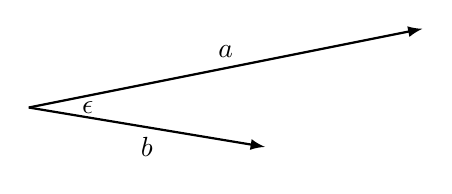
\begin{tikzpicture}
    \draw[-latex, thick] (0,0) -- node[above] {$\vv{a}$} (5,1);
    \draw[-latex, thick] (0,0) -- node[below] {$\vv{b}$} (3,-0.5);
    \node at (0.75,0)  {$\epsilon$};
\end{tikzpicture}
\end{center}
Bestimmen Sie einen Vektor in Richtung der Winkelhalbierenden des Winkels $\epsilon$!
\begin{answer}
Mit einerm Rhombus arbeiten: 
\[ \Vek{10}{-10}{17} \]
\end{answer}
\end{exercise}

\begin{exercise}
$A=(4/4/3)$, $B=(2/0/-1)$ \newline
In welchen Punkten durchstösst die $x$-Achse die Kugel mit Durchmesser $AB$?
\begin{answer}
Durchstosspunkte: $(1/0/0)$, $(5/0/0)$
\end{answer}
\end{exercise}

\begin{exercise}
$A=(4/-1/5)$, $B=(0/1/11)$, $C=(8/9/5)$, $D=(-2/-1/1)$ \newline
Zeigen Sie vektoriell, dass die Seitenmittelpunkte des Vierecks $ABCD$ ein Praallelogramm bilden.
\begin{answer}
Zu zeigen: Bezeichnet $PQRS$ das Viereck der Seitenmittelpunkte, so gilt $\vv{PQ} = \vv{SR}$.
\end{answer}
\end{exercise}

\begin{exercise}
$A=(1/2/3)$, $B=(4/3/1)$. Geben Sie folgende Vektoren bzw. Vektorbeträge an:
\begin{multicols}{2}
\begin{enumerate}
\item Ortsvektor des Punktes $A$
\item $\vv{AB}$
\item $\vv{BA}$
\item $3 \vv{AB}$
\item $|\vv{AB}|$
\item $|\vv{BA}|$
\end{enumerate}
\end{multicols}
Wie lauten die Koordinaten des Bildpunktes  bei einer Spiegelung von $A$
\begin{enumerate} 
\setcounter{enumii}{6}
\item an der $xy$-Ebene
\item an der $z$-Achse
\item am Ursprung?
\end{enumerate}

\begin{answer}
\begin{enumerate}
\item $\Vek{1}{3}{4}$
\item $\Vek{3}{1}{-2}$
\item $\Vek{-3}{-1}{2}$
\item $\Vek{9}{3}{-6}$
\item $\sqrt{14}$
\item $\sqrt{14}$
\item $(1/2/-3)$
\item $(-1/-2/3)$
\item $(-2/-2/-3)$
\end{enumerate}
\end{answer}
\end{exercise}

\begin{exercise}
$A=(-4/1/7)$, $B=(4/3/10)$, $C=(8/5/3)$ \newline
Bestimmen Sie den Punkt $D$ so, dass $ABCD$ ein Parallelogramm ist.
\begin{answer}
$\vv{OD} = \vv{OC} + \vv{BA} \rightarrow D=(0/3/0)$
\end{answer}
\end{exercise}

\begin{exercise}
$A=(1/1/4)$, $B=(6/3/0)$, $S=(4/0/3)$ \newline
Bestimmen Sie für das Dreieck $ABC$ mit dem Schwerpunkt $S$ die dritte Ecke $C$
\begin{answer}
$\vv{OC} = \vv{OM} + 3\vv{MS}$ mit $M=(3.5/2/2) \rightarrow C=(5/-4/5)$
\end{answer}
\end{exercise}

\begin{exercise}
$A=(3/0/5)$, $B=(7/7/10)$, $M=(5/6/6)$ \newline
$A$ und $B$ sind zwei Ecken und $M$ ist der Diagonalenschnittpunkt eines Parallelogramms $ABCD$. Bestimmen Sie die beiden anderen Ecken $C$ und $D$
\begin{answer}
$\vv{OC} = \vv{OM} + \vv{AM} \rightarrow C=(7/12/7)$, $\vv{OD} = \vv{OM} + \vv{BM} \rightarrow D=(3/5/2)$
\end{answer}
\end{exercise}

\begin{exercise}
Stellen Sie den Vektor $\vv{v}$ als Linearkombination von $\vv{a}$, $\vv{b}$ und $\vv{c}$ dar:
\begin{enumerate}
\item $\vv{a} = \Vek{2}{1}{-3}$, $\vv{b} = \Vek{-1}{1}{2}$, $\vv{c} = \Vek{2}{2}{-3}$, $\vv{v} = \Vek{1}{0}{-1}$
\item $\vv{a} = \Vek{-4}{2}{0}$, $\vv{b} = \Vek{-3}{1}{1}$, $\vv{c} = \Vek{1}{1}{-3}$, $\vv{v} = \Vek{5}{3}{1}$
\end{enumerate}
\begin{answer}
Gleichungssystem bestehend aus den drei Komponentengleichungen der Linearkombination $\vv{v} = x \vv{a} + y\vv{b} + z\vv{c}$ lösen.
\begin{enumerate}
\item $x=3$, $y=1$, $z=-2$
\item keine Lösung ($\vv{a}$, $\vv{b}$ und $\vv{c}$ sind komplanar, jedoch nicht $\vv{a}$, $\vv{b}$, $\vv{c}$ und $\vv{v}$).
\end{enumerate}
\end{answer}
\end{exercise}

\begin{exercise}
$A=(1/1/1)$, $B=(9/2/5)$, $C=(5/4/1)$ \newline
Berechnen Sie den Umfang $u$ des Dreiecks $ABC$.
\begin{answer}
$u=|\vv{AB}| + |\vv{BC}| + |\vv{CA}| = 20 $
\end{answer}
\end{exercise}

\begin{exercise}
Gegeben ist der Vektor $\vv{a} = \Vek{15}{-5}{7.5}$ \newline
Welches sind die zu $\vv{a}$ kolinearen Vektoren mit Betrag 7?
\begin{answer}
$|x \vv{a}| = 7 \Leftrightarrow |x| |\vv{a}| = 7 \Leftrightarrow x = \pm \frac{7}{|\vv{a}|} \rightarrow \Vek{6}{-2}{3}$, $\Vek{-6}{2}{-3}$
\end{answer}
\end{exercise}

\begin{exercise}
$A=(-1/1/0)$, $B=(-2/2/0)$, $C=2/1/-3)$ \newline
Welcher Punkt $P$ der $xy$-Ebene hat von jedem der drei Punkten $A$, $B$ und $C$ den gleichen Abstand?
\begin{answer}
$|\vv{AP}|= |\vv{BP}|$ und $|\vv{BP}|= |\vv{CP}|$ mit $P=(x/y/0) \rightarrow P=(2/5/0)$
\end{answer}
\end{exercise}

\end{exercisesKapitel}

